\paragraph{Probe on the clock-heldout checkpoint.} The pre-registered
test of whether the L1 linear axis is mechanical or task-driven
(PREREGISTRATION\_v2.md \S 2.1, anchor \texttt{80ddafc}). We
ran the same within-distribution probe (\texttt{model.qwen\_time\_probe\_within})
on the three \texttt{clock\_heldout\_s\{0,1,2\}.pt}
checkpoints (CLOCK supervision withheld during training, only
SILENT-GAP and PHASE seen). Across $n\,{=}\,3$ seeds:
$R^2(\text{L1}) = 0.99984 \pm 0.00007$ for the trained
model (condition A), and $R^2 = -0.00520 \pm 0.00000$ at
L1 for the $\alpha\,{=}\,0$ control (condition B). The
full-supervision baseline (\texttt{v15s\_s0}) is $R^2 = 0.99990$
at L1 by comparison. Pre-registered verdict at threshold
$R^2 \geq 0.99$: \textbf{MECHANICAL}. The linear $\tau$ axis at L1 is established by FiLM construction and one transformer block of processing, not by CLOCK-task supervision.
Figure~\ref{fig:probe-clock-heldout} overlays the per-layer curves.

\begin{figure}[!t]
  \centering
  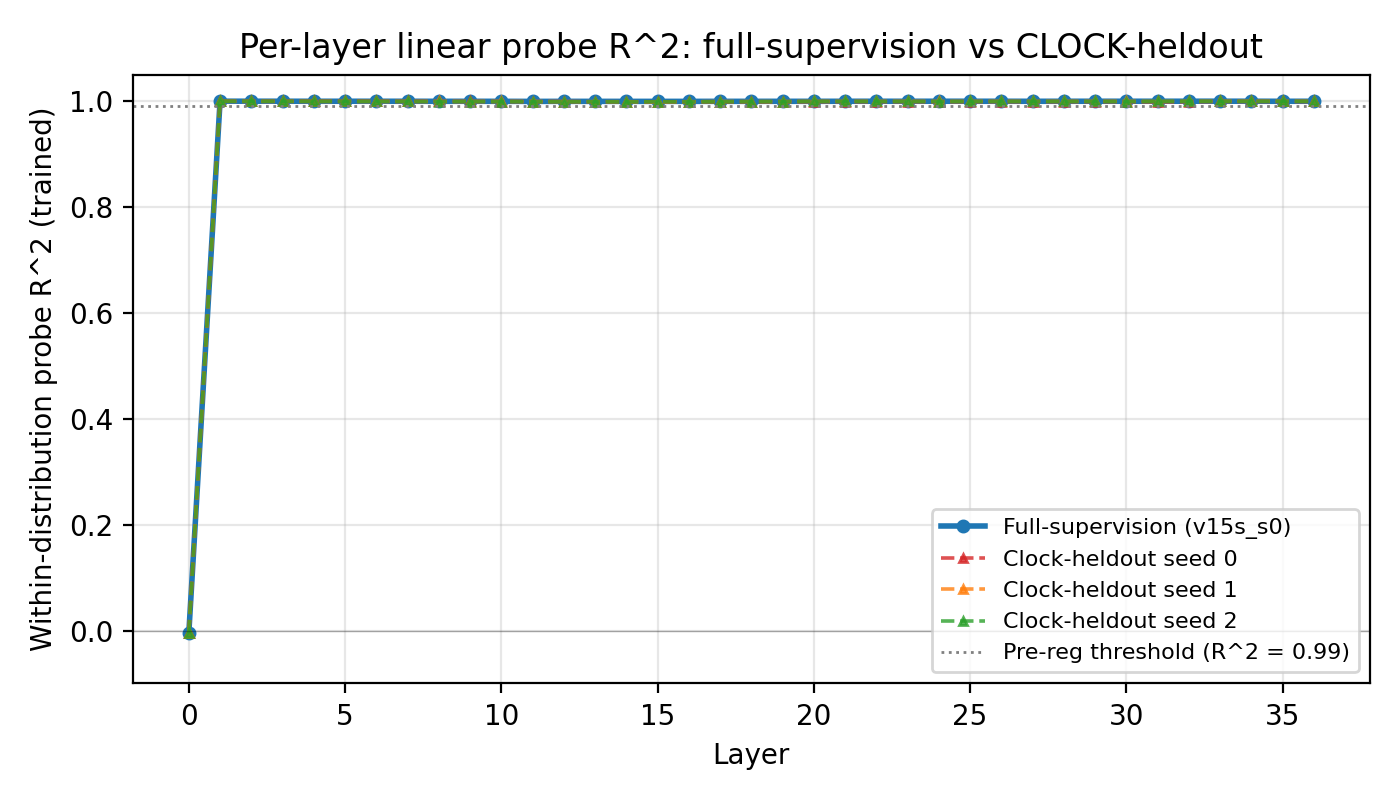
\includegraphics[width=\columnwidth]{figures/fig_probe_clock_heldout.png}
  \caption{Per-layer within-distribution probe $R^2$ vs.\ log$\tau$ on the
  full-supervision checkpoint (v15s\_s0, blue) and on the three
  CLOCK-heldout checkpoints (red/orange/green). Across $n\,{=}\,3$
  seeds, the linear axis at L1 survives removal of CLOCK supervision:
  $R^2 = 0.99984 \pm 0.00007$ for clock-heldout vs.\ $R^2 = 0.99990$
  for the full-supervision baseline. The axis is FiLM-mechanical, not
  CLOCK-task-driven. Pre-registered analysis: PREREGISTRATION\_v2.md
  section 2 (anchor \texttt{80ddafc}).}
  \label{fig:probe-clock-heldout}
\end{figure}
